\vspace{1em}
\begin{minipage}[t]{10cm}
  \vspace{-2cm}
  \section{Signal Modeling \hayes{129}}
  %\renewcommand{\arraystretch}{1.0}
  \textbf{Ziel: } Die Koeffizienten für ein Filter berechnen, dessen
  Impulsantwort möglichst genau mit einer gegebenen Signal ($x[n]$ - mit
  Länge $n$) übereinstimmt.
  
      $$ y(n) = \sum\limits_{k=0}^{q} b(k)x(n-k) - \sum\limits_{k=1}^{p} a(k)y(n-k)$$
      $$ H(z) = \dfrac{B(z)}{A(z)} = \dfrac{b_0 + b_1z^{-1} + b_2 z^{-2} + \dots +
      b_q z^{-q}}{1 + a_1z^{-1} + a_2 z^{-2} + \dots + a_p z^{-p}} $$ 

\end{minipage}
\hspace{0.25cm}
\begin{minipage}{9cm}
	\begin{tabular}{| p{1.4cm} | p{2cm} | p{3.9cm} | }
	    \hline
	    \textbf{Impuls\-antwort}
	    & exakte über\-ein\-stimmung
	    & kleinstes Fehler\-quadrat \\
	    \hline
	    \hline
	    \textbf{LS} 
	    & $[0]$
	    & $[1, n - 1]$\\
	    \hline
	    \textbf{Padé} 
	    & $[0, q + p + 1]$
	    & -\\
	    \hline
	    \textbf{Prony} 
	    & $[0, q]$
	    & $[q + 1, n-1]$ \\
	    \hline
	    \textbf{Shanks} 
	    & $[0]$
	    & $[1, n - 1]$\\
	    &&(zuerst a nach LS dann b. nicht beide zusammen)\\
	    \hline
	\end{tabular}\\
	$q$: Anzahl Nullstellen \hspace{1cm} $p$: Anzahl Polstellen
\end{minipage}

\subsection{Least Square Method \hayes{131}}
Die Koeffizienten \textbf{A und B} werden mit dem kleinsten Fehlerquadrat geschätzt. Da für die Schätzung ein $p+q$ Gleichungssystem aufgelöst 
werden muss, wird dies Methode sehr selten angewendet.\\
\begin{minipage}{8cm}
	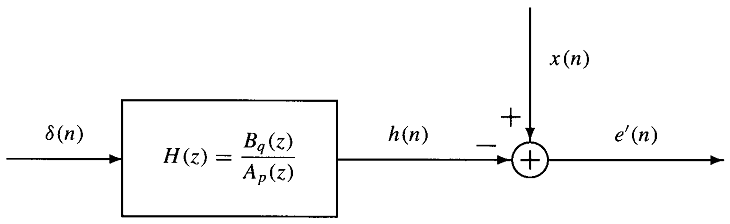
\includegraphics[width=8cm]{../StatDig/bilder/signalModeling.png}
\end{minipage}
\begin{minipage}{10cm}
$\frac{\partial \sum\limits_{n=0}^{\infty}|e'(n)|^2}{\partial a_p^*(k)}=\frac{1}{2\pi} \int\limits_{-\pi}^{\pi}\left[X(e^{j\omega})-
\frac{B_q(e^{j\omega})}{A_p (e^{j\omega})}\right]\frac{B^*_q(e^{j\omega})}{A_p^* (e^{j\omega})^2}e^{j\omega} d\omega=0$\\
$\frac{\partial \sum\limits_{n=0}^{\infty}|e'(n)|^2}{\partial b_q^*(k)}=\frac{1}{2\pi} \int\limits_{-\pi}^{\pi}\left[X(e^{j\omega})-
\frac{B_q(e^{j\omega})}{A_p (e^{j\omega})}\right]\frac{e^{j\omega}}{A_p^* (e^{j\omega})} d\omega=0$\\
\end{minipage} 
\subsubsection{Example FIR Equalizer}
With a FIR first order (2 coefficients) a given sequence (e.g. $[0, 2, 1, 0]$ ) should be filtered so that output is a Dirac $[0, 1 , 0 , 0]$.\\
$\underbrace{\begin{bmatrix}
x[0] 	& 0 	\\
x[1]	& x[0]	\\
0		& x[1]
\end{bmatrix}}_{\bm A}
\cdot \begin{bmatrix}
b_0\\
b_1
\end{bmatrix}=\begin{bmatrix}
1\\
0\\
0
\end{bmatrix}$. To solve the equations the pseudo inverse has to be used: $\bm A^{\dagger} = \left(\bm A^T \cdot \bm A\right)^{-1}\bm A^T 
\Rightarrow \bm  A^\dagger \begin{bmatrix}
1\\
0\\
0
\end{bmatrix}=\begin{bmatrix}
b_0\\
b_1
\end{bmatrix}$

\subsection{Padé Approximation \hayes{133}}
Resultierende Impulsantwort \textbf{stimmt} im Intervall $[0, q + p + 1]$ \textbf{exakt} mit
gegebenem Signal $x[n]$ überein, nachher ist der Filter nicht einmal zwingend stabil.

	%\vspace{-0.5cm}
	\renewcommand{\arraystretch}{1.0}
	\begin{aufzaehlung}
  		\item $a$-Koeffizienten / Pole berechnen: $\bm X_q \cdot a_p = -x_{q+1} \Longrightarrow a_p = - \bm X_q^{-1} \cdot x_{q+1}$ \matlab{$a_t = - X_t \backslash x$} \small $$
	%	\begin{matrix} n=q+1\\ n=q+2\\ \vdots \\ n=q+p \end{matrix}
		\underbrace{ \begin{bmatrix}
    		x[q]     & x[q-1]   & \hdots & x[q-p+1] \\                                   
    		x[q+1]   & x[q]     & \hdots & x[q-p+2] \\
    		\vdots   & \vdots   & \ddots & \vdots \\                             
    		x[q+p-1] & x[q+p-2] & \hdots & x[q] \\
		\end{bmatrix}  
		}_{\bm  X_q} \cdot 
		\underbrace{\begin{bmatrix}
    		a_1 \\
    		a_2 \\
    		\vdots \\
    		a_p
		\end{bmatrix}  }_{a_p} = \underbrace{\begin{bmatrix}
    		-x [q+1]\\            
    		-x [q+2]\\
    		\vdots \\
    		-x [q+p]\\
		\end{bmatrix}}_{x_{q+1}}  \Longleftrightarrow 
		\begin{bmatrix}
    		x[q+1] & x[q] & \hdots & x[q+1-p] \\                                   
    		x[q+2] & x[q+1] & \hdots & x[q+2-p] \\
    		\vdots & \vdots & \ddots & \vdots \\                             
    		x[q+p] & x[q+p-1] & \hdots & x[q] \\
		\end{bmatrix}
		\begin{bmatrix}
    		1 \\
    		a_1 \\
    		\vdots \\
    		a_p
		\end{bmatrix} = 
		\begin{bmatrix}
    		0 \\
    		0 \\
    		\vdots \\
    		0
		\end{bmatrix} 
		$$  \normalsize
		
		\vspace{-0.5cm}
		Falls A singulär ist, war die Annahme, dass $a_0 = 1$ falsch. $\Longrightarrow$ $a_0=0$ setzen. 
		$ \Longrightarrow \bm X_q \cdot \bm a_p = \bm 0$
		
  		\item $b$-Koeffizienten / Nullstellen berechnen: $\bm X_0 \cdot a_p = b_q$ \small \hspace{0.5cm}
		$ \begin{matrix} n=0\\ n=1\\ \vdots\\ n=q \end{matrix} \overset{(0 \hdots p)}{\underbrace{\begin{bmatrix}
    		x[0] & 0 & \hdots & 0 \\
    		x[1] & x[0] & \hdots & 0 \\
    		\vdots & \vdots & \ddots & \vdots \\
    		x[q] & x[q-1] & \hdots & x[q-p]
		\end{bmatrix}  }_{\bm X_0}}\cdot \underbrace{\begin{bmatrix}
    		1 \\
    		a_1 \\
    		\vdots \\
    		a_p
		\end{bmatrix}  }_{a_p}= 	\underbrace{\begin{bmatrix}
	    		b_0 \\
	    		b_1 \\
	    		\vdots \\
	    		b_q
			\end{bmatrix}}_{b_q}$ \normalsize
			
	\end{aufzaehlung}
	
\vspace{-1.0cm}


\subsection{Prony's Method \hayes{144}}
Resultierende Impulsantwort \textbf{stimmt} im Intervall $[0, q]$ \textbf{exakt} mit
gegebenem Signal $x[n]$ überein. Im Intervall $[q + 1, n-1]$ sind die
Werte mit dem \textbf{kleinsten Fehlerquadrat} (überbestimmtes GL-System)
angenähert. 

\renewcommand{\arraystretch}{1.0}

\begin{aufzaehlung}
	\item Autokorrelation berechnen: $ r_x(k,l) = \sum\limits_{n=q+1}^\infty x(n-l)x^*(n-k)$;\qquad $k,l\geq 0$
	\item $a$-Koeffizienten berechnen : $\bm R_x \cdot a_p = -r_x \Longrightarrow a_p = - \bm R_x^{-1} \cdot r_x$ 
  		\matlab{$a_p = - R_x \backslash r_x$} \small\\
		Der minimale Fehler ist: $\epsilon_{p,q} = r_x(0,0) + \sum\limits_{k=1}^p a_p(k) r_x(0,k)$
			$$
		\underbrace{\begin{bmatrix}
    		r_x[1,1] & r_x[1,2] & \hdots & r_x[1,p] \\                                   
    		r_x[2,1] & r_x[2,2] & \hdots & r_x[2,p] \\
    		\vdots & \vdots & \ddots & \vdots \\                             
    		r_x[p,1] & r_x[p,2] & \hdots & r_x[p,p] \\                        
		\end{bmatrix}  }_{\bm R_x} \cdot 
		\underbrace{\begin{bmatrix}
    		a_1 \\
    		\vdots \\
    		a_p
		\end{bmatrix}  }_{a_p}= -\underbrace{\begin{bmatrix}
    		r_x[1,0] \\
    		\vdots \\
    		r_x[p,0]
		\end{bmatrix}  }_{r_x}
		\Longrightarrow
		\begin{bmatrix}
    		r_x[0,0] & r_x[0,1] & \hdots & r_x[0,p] \\ 
    		----&----&----&----\\
    		r_x[1,0] & r_x[1,1] & \hdots & r_x[1,p] \\                                   
    		r_x[2,0] & r_x[2,1] & \hdots & r_x[2,p] \\
    		\vdots & \vdots & \ddots & \vdots \\                             
    		r_x[p,0] & r_x[p,1] & \hdots & r_x[p,p] \\                        
		\end{bmatrix} \cdot 
		\begin{bmatrix}
    		1 \\
    		a_1 \\
    		\vdots \\
    		a_p
		\end{bmatrix} = \begin{bmatrix}
    		\epsilon_{p,q} \\
    		---\\
    		0 \\
    		\vdots \\
    		0
		\end{bmatrix} $$ 
		Für All-Pole Modelle können die a-Koeffizienten direkt aus dem b Gleichungsystem berechnet werden. 
		Dafür müssen alle $b$-Koeffizienten bis auf $b_0$ auf 0 gesetzt werden.
	\item $b$-Koeffizienten berechnen wie bei \textbf{Padé}: $\bm X_0 \cdot a_p = b_q$ 
		\normalsize
\end{aufzaehlung}
	
\subsection{Shanks' Method \hayes{154}}

Die B Koeffizient werden bei gegebenen A's so geschätzt, dass die resultierende Impulsantwort ist im Intervall $[0, n - 1]$ mit dem
\textbf{kleinsten Fehlerquadrat} (überbestimmtes GL-System) dem gegebenen
Signal $x[n]$ angenähert wird. Die einzige Verbesserung wäre noch wenn die A- Koeffizenten auch noch alle Signalwerte einbeziehen würden (Least-square).

\begin{aufzaehlung}
  		\item $a$-Koeffizienten berechnen wie bei \textbf{Prony}: $a_p = - \bm R_x^{-1} \cdot r_x$ \matlab{$a_p = - R_x \backslash r_x$}  
  		\item Impulsantwort $g[n]$ des rein rekursiven Filters ($g[n] = \delta(n)- \sum\limits_{k=1}^p a_p(k)g(n-k)$) berechnen, 
  		oder mittels inversen z-Transformation von $H(z)$.
  		\item Autokorrelation berechenen:  $r_g(k)=\sum\limits_{n=0}^\infty g(n)g^*(n-k)$; oder inverse z-Transformation von $|H(z)|^2$
  		\item Kreuzkorrelation berechnen: $r_{xg}(k)=\sum\limits_{n=0}^\infty x(n)g^*(n-k)$
  		\item $b$-Koeffizienten berechnen (für stationäre Prozesse): $b_q = R_g^{-1} \cdot r_{xg}$ \matlab{$b_q = R_g \backslash r_{xg}$}\\
  		für\\
  		
			
		 $$\begin{matrix}n=0\\ n=1\\ \vdots\\ n=N_{ha}+q\\ \end{matrix}
		\overset{(0 \hdots q)}{\underbrace{\begin{bmatrix}
    		r_g(0) & r_g(1) & \hdots & r_g(q) \\                                            
    		r_g(1) & r_g(0) & \hdots & r_g(q-1) \\         
    		\vdots & \vdots & \ddots & \vdots \\                                      
    		r_g(q) &r_g(q-1) & \hdots & r_g(0) \\    
		\end{bmatrix}  }_{R_g}} \cdot \underbrace{\begin{bmatrix}
    		b_0 \\
    		b_1 \\
    		\vdots \\
    		b_q
		\end{bmatrix}  }_{b_q}= \underbrace{\begin{bmatrix}
    		r_{xg}(0) \\
    		r_{xg}(1) \\
    		\vdots \\
    		r_{xg}(q) \\
		\end{bmatrix}  }_{r_{gx}} $$
\end{aufzaehlung}

\newpage
\subsection{All-Pole Modeling \hayes{160}}
Entspricht: \ref{sec:autoregressive_model_method}
\begin{aufzaehlung}
	\item Autokorrelation berechnen: $ r_x(k) = \sum\limits_{n=0}^\infty x(n)x^*(n-k)$;\qquad $k\geq 0$
	\item $a$-Koeffizienten berechnen : $\bm R_x \cdot a_p = -r_x \Longrightarrow a_p = - \bm R_x^{-1} \cdot r_x$ 
  		\matlab{$a_p = - R_x \backslash r_x$} \small\\
		Der minimale Fehler ist: $\epsilon_{p,q} = r_x(0) + \sum\limits_{k=1}^p a_p(k) r_x(k)$
			$$
		\underbrace{\begin{bmatrix}
    		r_x(0) & r_x(1) & \hdots & r_x(p-1) \\                                   
    		r_x(1) & r_x(0) & \hdots & r_x(p-2) \\
    		\vdots & \vdots & \ddots & \vdots \\                             
    		r_x(p-1) & r_x(p-2) & \hdots & r_x(0) \\                        
		\end{bmatrix}  }_{\bm R_x} \cdot 
		\underbrace{\begin{bmatrix}
    		a_1 \\
    		\vdots \\
    		a_p
		\end{bmatrix}  }_{a_p}= -\underbrace{\begin{bmatrix}
    		r_x(1) \\
    		\vdots \\
    		r_x(p)
		\end{bmatrix}  }_{r_x}$$ 
	\item $b(0) = \sqrt{\epsilon_p}$ 
\end{aufzaehlung}

\subsection{Linear Prediction \hayes{165} sowie Aufgabe 4.13}

		$$\hat{x}(n+n_0) = \sum\limits_{k=1}^p a_p(k) x(n-k)$$
		$$
		\underbrace{\begin{bmatrix}
    		r_x[1,1] & r_x[1,2] & \hdots & r_x[1,p] \\                                   
    		r_x[2,1] & r_x[2,2] & \hdots & r_x[2,p] \\
    		\vdots & \vdots & \ddots & \vdots \\                             
    		r_x[p,1] & r_x[p,2] & \hdots & r_x[p,p] \\                        
		\end{bmatrix}  }_{\bm R_x} \cdot 
		\underbrace{\begin{bmatrix}
    		a_1 \\
    		\vdots \\
    		a_p
		\end{bmatrix}  }_{a_p}= \underbrace{\begin{bmatrix}
    		r_x[1,-n_0] \\
    		\vdots \\
    		r_x[p,-n_0]
		\end{bmatrix}  }_{r_x}$$

\subsection{FIR Inverse Filter \hayes{166}}
$$G(z)H(z) \approx 1\qquad g(n)*h(n) \approx \delta(n) \qquad r_g(k) = \sum\limits_{n=0}^\infty g(n)g^*(n-k) \qquad \text{Delay: } n_0$$

		$$
		\underbrace{\begin{bmatrix}
    		r_g(0) & r_g(1) & \hdots & r_g(N-1) \\                                   
    		r_g(1) & r_g(0) & \hdots & r_g(N-2) \\
    		\vdots & \vdots & \ddots & \vdots \\                             
    		r_g(N-1) & r_g(N-2) & \hdots & r_g(0) \\                        
		\end{bmatrix}  }_{\bm R_g} \cdot 
		\underbrace{\begin{bmatrix}
    		h_N(0) \\
    		\vdots \\
    		h_N(N-1)
		\end{bmatrix}  }_{h_N}= -\underbrace{\begin{bmatrix}
    		g(n_0) \\
    		g(n_0 - 1)	 \\
    		\vdots \\
    		g(0)\\
    		0\\
    		\vdots \\
    		0
		\end{bmatrix}  }_{r_{gd}}$$

\clearpage
\subsection{Approximation mit begrenzten  Daten mit All-Pole Filter}
\subsubsection{Autocorrelation Method \hayes{178}}
Sind die die Autokorrellationen gegeben, siehe Kapitel \ref{sec:autoregressive_model_method}.\\
Annahme: Die Daten $x[n]$ sind ausserhalb des Definitionsbereichs ($n=[0..N]$) Null: $x[n]=0$. So wird der Filter in einen stabilen Zustand gezwungen.
\renewcommand{\arraystretch}{1.0}

\begin{aufzaehlung}
	\item $a$-Koeffizienten berechnen (mittels Pseudoinverse / generalisierte Inverse): $a_p = -\left(\bm X_p^T \cdot \bm  X_p\right)^{-1} \cdot \bm X_p^T \cdot x_1$
  		\matlab{$a_p = -X_p \backslash x_1$} \small
			$$
		\begin{matrix} n=q+1\\ n=q+2\\ \vdots \\ n=N\\ n=N+1\\ \vdots \\ N+p
		\end{matrix}
		\underbrace{\begin{bmatrix}
    		x[0] & 0 & \hdots & 0 \\ 
    		x[1] & x[0] & \hdots & 0 \\ 
    		x[2] & x[1] & \hdots & 0 \\        
    		\vdots & \vdots & \ddots & \vdots \\
    		----&----&----&----\\                
    		x[p-1] & x[p-2] & \hdots & x[0] \\                                   
    		x[p] & x[p-1] & \hdots & x[1] \\      
    		\vdots & \vdots & \ddots & \vdots \\                        
    		x[N-1] & x[N-2] & \hdots & x[N-p] \\ 
    		----&----&----&----\\                            
    		x[N] & x[N-1] & \hdots & x[N-p+1] \\ 
    		0 & x[N] & \hdots & x[N+2-p] \\
    		\vdots & \vdots & \ddots & \vdots \\                     
    		0 & 0 & \hdots & x[N] \\
		\end{bmatrix}  }_{\bm X_p=(N+p \; \times \; p) Matrixe} \cdot \underbrace{\begin{bmatrix}
    		a_1 \\
    		\vdots \\
    		a_p
		\end{bmatrix}  }_{a_p}= \underbrace{\begin{bmatrix}
    		 -x [1]\\            
    		 -x [2]\\
    		\vdots \\
    		 -x [N]\\
    		0 \\
    		\vdots \\
    		0
		\end{bmatrix}}_{x_1} 
		 $$ \normalsize
	\end{aufzaehlung}
	
\subsubsection{Covariance Method  \hayes{183}}
Es werden keine Annahmen getroffen, nur die vorhanden Daten werden verwendet. Der Nachteil ist, dass das Filter instabil werden kann. 
Ein weiterer Nachteil ist, dass A keine Toeplitz Matrixe ist, so dass das Auflösen nicht so einfach ist wie bei der Autokorrelation Methode. 
Das Signal wird jedoch genauer rekonstruiert. Bei einer Datenreihe, welche einer Impulsantwort entspricht, wird der Filter perfekt rekonstruiert. 
Mit dem Nachteil, dass auch die instabilen Pole implementiert werden. $a_p = -\left(\bm X_p^T \cdot \bm  X_p\right)^{-1} \cdot \bm X_p^T \cdot x_p$ \matlab{$a_p = -X_p \backslash x_p$} \small
		$$
		\underbrace{\begin{bmatrix}               
    		x[p-1] & x[p-2] & \hdots & x[0] \\                                   
    		x[p] & x[p-1] & \hdots & x[1] \\      
    		\vdots & \vdots & \ddots & \vdots \\                        
    		x[N-1] & x[N-2] & \hdots & x[N-p] \\ 
		\end{bmatrix}  }_{\bm X_p} \cdot \underbrace{\begin{bmatrix}
    		a_1 \\
    		\vdots \\
    		a_p
		\end{bmatrix}  }_{a_p}= \underbrace{\begin{bmatrix}
    		 -x[p]\\            
    		 -x[p+1]\\
    		\vdots \\
    		 -x[N]\\
		\end{bmatrix}}_{x_p} 
		 $$ \normalsize
\vspace{-0.6cm}

\subsection{Stochastische Modelle}
Bei stochastischen Modellen werden generell die gleichen Modelle verwendet, wie in der deterministischen Welt. 
Anstatt des Dirac-Impulses wird weisses Rauschen am Eingang des Filters verwendet und die Autokorrelation wird mit Hilfe des Erwartungswertes gebildet. 
$r(k)=E\{x(n) \cdot x^*(n-k)\}$\\
Anstatt der Kreuzkorellation $r_{gx}$ wird die Faltung von $b_q(k)$ und $h^*(-k)$ verwendet. $c_q(k) = b_q(k) \ast h^*(-k)$

\subsubsection{Autoregressive Moving Average Models, ARMA \hayes{189}}
Ein ARMA Pozess ist weisses Rauschen welches durch ein LTI- System $H(z)$ gefiltert wird.\\
Um die Koeffizienten von $H(z)=\frac{B_q(z)}{A_p(z)}=\frac{\sum\limits_{k=0}^q b_q(k)z^{-k}}{1+\sum\limits_{k=1}^p a_p(k)z^{-k}}$ werden 
die \textbf{erweiterten Yule-Walker Gleichungen} gelöst:
\small$$
\underbrace{\begin{bmatrix}               
    		r_x[0] & r_x^*[1] & \hdots & r_x^*[p] \\   
    		r_x[1] & r_x^*[0] & \hdots & r_x^*[p-1] \\   
    		\vdots & \vdots & \ddots & \vdots \\     
    		r_x[q] & r_x[q-1] & \hdots & r_x[q-p] \\   
    		r_x[q+1] & r_x[q] & \hdots & r_x[q-p+1] \\    
    		\vdots & \vdots & \ddots & \vdots \\     
    		r_x[L] & r_x[L-1] & \hdots & r_x[L-p] \\ 
		\end{bmatrix}  }_{R_x} \cdot \underbrace{\begin{bmatrix}
    		1\\
    		a_p(1) \\
    		a_p(2) \\
    		\vdots \\
    		a_p(p)
		\end{bmatrix}  }_{a_p}= \begin{bmatrix}
    		 c_q[0]\\            
    		 c_q[1]\\
    		\vdots \\
    		 c_q[q]\\
    		 0\\
    		\vdots \\
    		 0\\
		\end{bmatrix} 
		 $$ \normalsize

\begin{aufzaehlung}
  		\item Berechnen der A- Koeffizienten: $R_q \cdot a_p = - r_{q+1}$
  		\small$$
\underbrace{\begin{bmatrix}                   
    		r_x[q] & r_x[q-1] & \hdots & r_x[q-p+1] \\   
    		r_x[q+1] & r_x[q] & \hdots & r_x[q-p+2] \\    
    		\vdots & \vdots & \ddots & \vdots \\     
    		r_x[q+p-1] & r_x[q+p-2] & \hdots & r_x[q] \\ 
		\end{bmatrix}  }_{R_q} \cdot \underbrace{\begin{bmatrix}
    		a_p(1) \\
    		a_p(2) \\
    		\vdots \\
    		a_p(p)
		\end{bmatrix}  }_{a_p}= \underbrace{\begin{bmatrix}
    		 -r_x[q+1]\\            
    		 -r_x[q+2]\\
    		\vdots \\
    		 -r_x[q+p]\\
		\end{bmatrix}}_{r_{q+1}} 
		 $$ \normalsize
		 \item Zur Berechnung der B- Koeffizienten muss der Umweg über die C- Koeffizienten genommen werden: $R_x \cdot a_p = c_q$
	
  		\small$$
\underbrace{\begin{bmatrix}                   
    		r_x[0] & r_x^*[1] & \hdots & r_x^*[p] \\   
    		r_x[1] & r_x[0] & \hdots & r_x^*[p-1] \\    
    		\vdots & \vdots & \ddots & \vdots \\     
    		r_x[q] & r_x[q+1] & \hdots & r_x[0] \\ 
		\end{bmatrix}  }_{R_x} \cdot \underbrace{\begin{bmatrix}
			1 \\
    		a_p(1) \\
    		a_p(2) \\
    		\vdots \\
    		a_p(p)
		\end{bmatrix}  }_{a_p}= - \underbrace{\begin{bmatrix}
    		 c_q[0]\\            
    		 c_q[1]]\\
    		\vdots \\
    		 c_q[q]\\
		\end{bmatrix}}_{c_{q}} 
		 $$ \normalsize	 
		 \item $[C_q(z)]_+$ aufschreiben: $[C_q(z)]_+ = \sum\limits_{k=0}^q c_q(k)z^{-k}$
		 \item $[P_y(z)]_+=\left[[C_q(z)]_+ \cdot A^*_p(1/z^*)\right]_+$ berechnen. \\
		 z.B $[C_1(z)]_+=\frac{45}{2}-6z^{-1}$, $A^*_p(1/z^*)=1-0.5z$; $[C_1(z)]_+ \cdot A^*_p(1/z^*)= -\frac{45}{4}z +\frac{51}{2}-6z^{-1}$ $\Rightarrow$  $[P_y(z)]_+= \frac{51}{2}-6z^{-1}$
		 \item $[P_y(z)]_+$ symterisch machen. z.B: $P_y(z) =  -6 z +\frac{51}{2}-6z^{-1}$
		 \item Faktorisieren von $P_y(z)=B_q(z)B_q^*(1/z^*)$ damit $B_p(z)$ verwendet werden kann: \\
		 z.B. $B_1(z)\cdot B_1^*(1/z^*)= \underbrace{2\sqrt{6}(1-\frac{1}{4}z^{-1})}_{B_q(z)}\cdot \underbrace{2\sqrt{6}(1-\frac{1}{4}z^{1})}_{B_q^*(1/z^*)}$
		 \item $H(z)=\frac{B_q(z)}{A_p(z)}$ z.B: $H(z)=\frac{2 \sqrt{6}(1-\frac 1 4 z^{-1})}{A_p(z)}$
\end{aufzaehlung}
		 
\subsubsection{Autoregressive Models - AR \hayes{194}}
\label{sec:autoregressive_model_method}
Bei der AR wird die ARMA Methode verwendet, jedoch nur mit Polen. $H(z)=\frac{b(0)}{1+\sum\limits_{k=1}^{p} a_p(k)z^{-k}}$.\\
 $$\begin{bmatrix} 
	 	r_x(0)  & r_x^*(1) & r_x^*(2) & \cdots & r_x^*(p-1)\\
	 	r_x(1)  & r_x(0) & r_x^*(1) & \cdots & r_x^*(p-2)\\
	 	r_x(2)  & r_x(1) & r_x(0) & \cdots & r_x^*(p-3)\\
	 	\vdots  & \vdots  & \vdots  & \vdots & \vdots\\
	 	r_x(p-1)& r_x(p-2)& r_x(p-3)& \cdots &  r_x(0)\\
   \end{bmatrix}=
   \begin{bmatrix}
    	a_p(1)\\
    	a_p(2)\\
    	a_p(3)\\
    	\vdots\\
    	a_p(p)\\
   \end{bmatrix}=
   \begin{bmatrix}
       	-r_x(1)\\
       	-r_x(2)\\
       	-r_x(3)\\
       	\vdots\\
        -r_x(p)\\
   \end{bmatrix}
 $$
 Mit $|b(0)|^2=r_x(0) + \sum\limits_{k=1}^{p} a_p(k)r_x(k)$
 

 
 \subsubsection{Moving Average Models - MA \hayes{195}}
Ein MA Prozess ist eine Spezialform von einem ARMA Prozess, welcher nur Nullstellen besitzt.\\
$P_x(z)=\sum\limits_{k=-q}^{q}r_x(k)z^{-k}=B_q(z)B_q^*(1/z^*)$
\begin{aufzaehlung}
	\item $P_x(z)$ spektral faktorisieren in: $P_x(z)=\sigma^2_0 \cdot Q(z)\cdot Q^*(1/z^*)=\underbrace{\sigma^2_0}_{|b_q(0)|^2} \underbrace{\prod\limits_{k=1}^q (1-\beta_k z^{-1})}_{B_q(z)} \cdot \underbrace{\prod\limits_{k=1}^q (1-\beta_k^* z)}_{B^*_q(1/z^*)}$
	\item $B_q(z)$ ausmultiplizieren $\Rightarrow$ minimum phase filter (alle Nullstellen sind innerhalb des Einheitskreis)
	\item bzw. $B_q^*(1/z^*)$ ausmultiplizieren ergibt ein maximum phase filter (alle Nullstellen sind ausserhalb des Einheitskreis)
\end{aufzaehlung}
